\documentclass[12pt]{article}
\usepackage[a4paper total={10in, 10in}]{geometry}
\usepackage[myheadings]{fullpage}
\usepackage{fancyhdr}
\usepackage{lastpage}
\usepackage{graphicx}
\usepackage[T1]{fontenc}
\usepackage[font=small, labelfont=bf]{caption}
\usepackage{fourier}
\usepackage[protrusion=true, expansion=true]{microtype}
\usepackage[english]{babel}
\usepackage{sectsty}
\usepackage{url, lipsum}
\usepackage{tgbonum}
\usepackage{hyperref}
\usepackage{xcolor}
\usepackage{listings}
\usepackage{listings-rust}
\usepackage{textcomp}
\usepackage{datetime}
\usepackage{multicol}
\usepackage{multirow}

\newcommand\tab[1][1cm]{\hspace*{#1}}
\newcommand{\HRule}[1]{\rule{\linewidth}{#1}}
\setcounter{tocdepth}{5}
\setcounter{secnumdepth}{5}

\pagestyle{fancy}
\fancyhf{} 
\fancyhead[L]{Lexical Analysis}
\fancyhead[C]{CP471 - Phase 1}
\fancyhead[R]{02.27.23}
\fancyfoot[C]{\thepage}

\usepackage{listings}
\usepackage{color}
\definecolor{dkgreen}{rgb}{0,0.6,0}
\definecolor{gray}{rgb}{0.5,0.5,0.5}
\definecolor{mauve}{rgb}{0.58,0,0.82}

\usepackage{tikz}
\usepackage{pgfplots}
\usetikzlibrary{datavisualization}
% \pgfplotsset{compat=1.9}
% \usepgfplotslibrary{external}
% \tikzexternalize

\lstset{frame=tb,
  language=Rust,
  aboveskip=3mm,
  belowskip=3mm,
  showstringspaces=false,
  columns=flexible,
  basicstyle={\small\ttfamily},
  numbers=none,
  numberstyle=\tiny\color{gray},
  keywordstyle=\color{blue},
  commentstyle=\color{dkgreen},
  stringstyle=\color{mauve},
  breaklines=true,
  breakatwhitespace=true,
  tabsize=3
}

\begin{document} {
    % ------------- COVER PAGE -------------
    \fontfamily{put}\selectfont
    \title
    { 
        \normalsize \textsc{}
        \\ [2.0cm]
        \HRule{3pt} \\
        \LARGE \textbf
        {
            {
                CP471 - Intro to Compiling \\
                Phase \#1 \\
            }
            \HRule{3pt} \\ [0.5cm]
            \textbf{\LARGE{Topic: Lexical Analysis}}
        }
    }
    
    \author {
    	Aidan Traboulay
	}
    
    \date {
        \textbf{\today}
    }
    
    \maketitle
    % ------------- INTRO --------------
    \newpage
    \section {Introduction}
    The initial stage of a compiler is called lexical analysis, and it has a fundamental role in converting a high-level programming language into machine language that can be understood by computers. This stage involves examining the program's source code and breaking it down into distinct "tokens," which are the fundamental components of the programming language. These tokens are then evaluated and sorted according to their classification, including keywords, identifiers, operators, and literals. The primary objective of this phase is to transform the original source code into a well-organized set of tokens that can be effortlessly handled by the following phase of the compiler, which is the parser.

    % ------------- Grammar --------------
    \newpage
    \section {Grammar}
    \begin{lstlisting}[language={}]
<program> ::= <fdecls> <declarations> <statement_seq>.
<fdecls> ::= <fdec>; | <fdecls> <fdec>; |
<fdec> ::= def <type> <fname> ( <params> ) <declarations> <statement_seq> fed
<params> ::= <type> <var> | <type> <var> , <params> |
<fname> ::= <id>
<declarations> ::= <decl>; | <declarations> <decl>; |
<decl> := <type> <varlist>
<type> := int | double
<varlist> ::= <var>, <varlist> | <var>
<statement_seq> ::= <statement> | <statement>; <statement_seq>
<statement> ::= <var> = <expr> |
if <bexpr> then <statement_seq> fi |
if <bexpr> then <statement_seq> else <statement_seq> fi |
while <bexpr> do <statement_seq> od |
print <expr> |
return <expr> |
<expr> ::= <expr> + <term> | <expr> - <term> | <term>
<term> ::= <term> * <factor> | <term> / <factor> | <term> % <factor> |
<factor>
<factor> ::= <var> | <number> | (<expr>) | <fname>(<exprseq>)
<exprseq> ::= <expr>, <exprseq> | <expr> |
<bexpr> ::= <bexpr> or <bterm> | <bterm>
<bterm> ::= <bterm> and <bfactor> | <bfactor>
<bfactor> ::= (<bexpr>) | not <bfactor> | (<expr> <comp> <expr>)
<comp> ::= < | > | == | <= | >= | <>
<var> ::= <id> | <id>[<expr>]
<letter> ::= a | b | c | ... | z
<digit> ::= 1 | 2 | 3 | 4 | 5 | 6 | 7 | 8 | 9 | 0
<id> ::= <letter> | <id><letter> | <id><digit>
<number> ::= <integer> | <double>...
    \end{lstlisting}

    % ------------- Terminals & Non-Terminals --------------
    \newpage
    \section {Terminals \& Non-Terminals}
    \begin{multicols}{2}
    Non-Terminals
    \begin{lstlisting}[language={}]
<program>
<fdecls>
<fdec>
<params>
<fname>
<declarations>
<decl>
<type>
<varlist>
<statement_seq>
<statement>
<expr>
<term>
<factor>
<exprseq>
<bexpr>
<bterm>
<bfactor>
<comp>
<var>
<letter>
<digit>
<id>
<number>
ㅤ
ㅤ
ㅤ
ㅤ
ㅤ
ㅤ
    \end{lstlisting}
    \columnbreak
    Terminals
    \begin{lstlisting}[language={}]
def
fed
(
)
,
int
double
=
if
then
else
while
do
od
print
return
/
%
or
and
not
<
==
<=
=
<>
[
]
a, b, c, ..., z (lowercase)
1, 2, 3, 4, 5, 6, 7, 8, 9, 0 (digits)
    \end{lstlisting}
    \end{multicols}
    % ------------- DFA --------------
    \newpage
    \section {Deterministic Finite Automaton}
    \subsection{State Diagram}
    \begin{center}
        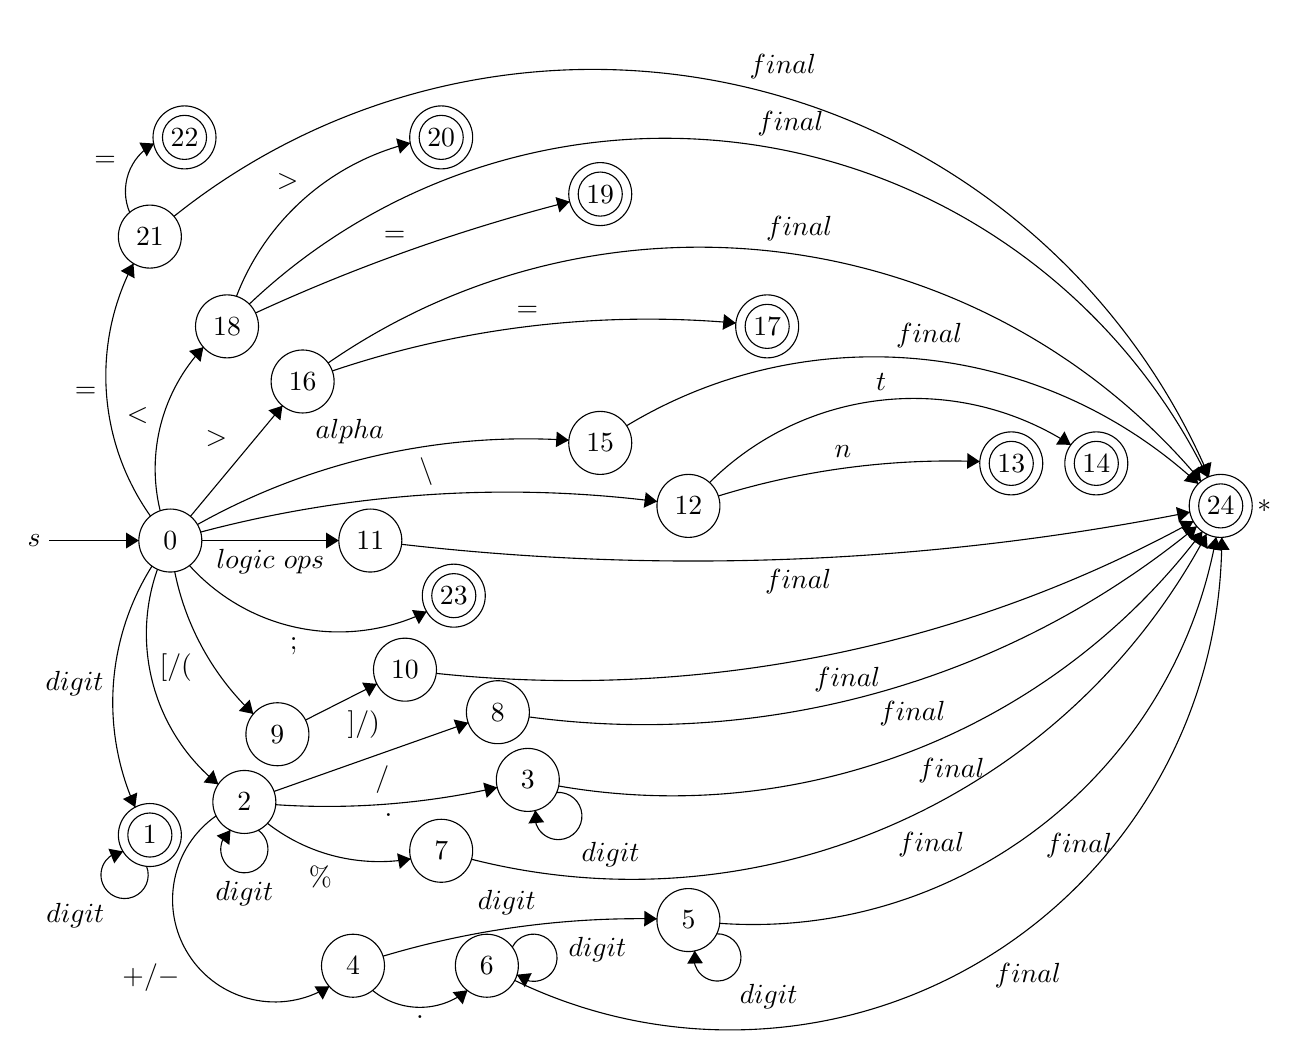
\begin{tikzpicture}[scale=0.2]
        \tikzstyle{every node}+=[inner sep=0pt]
        \draw [black] (8,-29.3) circle (2);
        \draw (8,-29.3) node {$0$};
        \draw [black] (74.7,-27.1) circle (2);
        \draw (74.7,-27.1) node {$24$};
        \draw (77,-27.1) node [right] {$*$};
        \draw [black] (74.7,-27.1) circle (1.4);
        \draw [black] (6.7,-48) circle (2);
        \draw (6.7,-48) node {$1$};
        \draw [black] (6.7,-48) circle (1.4);
        \draw [black] (12.7,-45.9) circle (2);
        \draw (12.7,-45.9) node {$2$};
        \draw [black] (30.7,-44.5) circle (2);
        \draw (30.7,-44.5) node {$3$};
        \draw [black] (19.6,-56.3) circle (2);
        \draw (19.6,-56.3) node {$4$};
        \draw [black] (40.9,-53.4) circle (2);
        \draw (40.9,-53.4) node {$5$};
        \draw [black] (28.1,-56.3) circle (2);
        \draw (28.1,-56.3) node {$6$};
        \draw [black] (6.7,-10) circle (2);
        \draw (6.7,-10) node {$21$};
        \draw [black] (8.9,-3.7) circle (2);
        \draw (8.9,-3.7) node {$22$};
        \draw [black] (8.9,-3.7) circle (1.4);
        \draw [black] (11.6,-15.7) circle (2);
        \draw (11.6,-15.7) node {$18$};
        \draw [black] (16.4,-19.2) circle (2);
        \draw (16.4,-19.2) node {$16$};
        \draw [black] (25.2,-3.7) circle (2);
        \draw (25.2,-3.7) node {$20$};
        \draw [black] (25.2,-3.7) circle (1.4);
        \draw [black] (40.9,-27.1) circle (2);
        \draw (40.9,-27.1) node {$12$};
        \draw [black] (61.4,-24.4) circle (2);
        \draw (61.4,-24.4) node {$13$};
        \draw [black] (61.4,-24.4) circle (1.4);
        \draw [black] (66.8,-24.4) circle (2);
        \draw (66.8,-24.4) node {$14$};
        \draw [black] (66.8,-24.4) circle (1.4);
        \draw [black] (35.3,-7.3) circle (2);
        \draw (35.3,-7.3) node {$19$};
        \draw [black] (35.3,-7.3) circle (1.4);
        \draw [black] (35.3,-23.1) circle (2);
        \draw (35.3,-23.1) node {$15$};
        \draw [black] (45.9,-15.7) circle (2);
        \draw (45.9,-15.7) node {$17$};
        \draw [black] (45.9,-15.7) circle (1.4);
        \draw [black] (25.2,-49) circle (2);
        \draw (25.2,-49) node {$7$};
        \draw [black] (28.8,-40.2) circle (2);
        \draw (28.8,-40.2) node {$8$};
        \draw [black] (20.7,-29.3) circle (2);
        \draw (20.7,-29.3) node {$11$};
        \draw [black] (14.8,-41.6) circle (2);
        \draw (14.8,-41.6) node {$9$};
        \draw [black] (22.9,-37.5) circle (2);
        \draw (22.9,-37.5) node {$10$};
        \draw [black] (26,-32.8) circle (2);
        \draw (26,-32.8) node {$23$};
        \draw [black] (26,-32.8) circle (1.4);
        \draw [black] (5.77,-46.231) arc (-155.80682:-212.14664:16.251);
        \fill [black] (5.77,-46.23) -- (5.9,-45.3) -- (4.99,-45.71);
        \draw (3.78,-38.4) node [left] {$digit$};
        \draw [black] (6.489,-49.981) arc (21.65207:-266.34793:1.5);
        \draw (1.96,-52.3) node [below] {$digit$};
        \fill [black] (5,-49.04) -- (4.07,-48.87) -- (4.44,-49.8);
        \draw [black] (13.582,-47.686) arc (54:-234:1.5);
        \draw (12.7,-50.9) node [below] {$digit$};
        \fill [black] (11.82,-47.69) -- (10.94,-48.04) -- (11.75,-48.63);
        \draw [black] (18.095,-57.605) arc (-57.87352:-235.00099:6.498);
        \fill [black] (18.1,-57.61) -- (17.15,-57.61) -- (17.68,-58.45);
        \draw (8.61,-57.03) node [left] {$+/-$};
        \draw [black] (28.759,-44.98) arc (-77.27834:-93.82689:49.019);
        \fill [black] (28.76,-44.98) -- (27.87,-44.67) -- (28.09,-45.64);
        \draw (21.85,-46.59) node [below] {$.$};
        \draw [black] (11.048,-44.776) arc (-128.89035:-199.49256:12.278);
        \fill [black] (11.05,-44.78) -- (10.74,-43.88) -- (10.11,-44.66);
        \draw [black] (32.527,-45.295) arc (94.2019:-193.7981:1.5);
        \draw (35.95,-48.43) node [below] {$digit$};
        \fill [black] (31.18,-46.43) -- (30.74,-47.27) -- (31.74,-47.19);
        \draw [black] (73.535,-28.725) arc (-36.98825:-99.85866:42.139);
        \fill [black] (73.54,-28.73) -- (72.65,-29.06) -- (73.45,-29.67);
        \draw (57.59,-43.1) node [below] {$final$};
        \draw [black] (0.3,-29.3) -- (6,-29.3);
        \draw (-0.2,-29.3) node [left] {$s$};
        \fill [black] (6,-29.3) -- (5.2,-28.8) -- (5.2,-29.8);
        \draw [black] (21.506,-55.693) arc (106.65494:88.85139:56.728);
        \fill [black] (38.9,-53.32) -- (38.11,-52.81) -- (38.09,-53.81);
        \draw (29.36,-53.12) node [above] {$digit$};
        \draw [black] (42.691,-54.273) arc (91.75396:-196.24604:1.5);
        \draw (45.99,-57.45) node [below] {$digit$};
        \fill [black] (41.3,-55.35) -- (40.82,-56.17) -- (41.82,-56.14);
        \draw [black] (26.868,-57.857) arc (-50.43979:-129.56021:4.739);
        \fill [black] (26.87,-57.86) -- (25.93,-57.98) -- (26.57,-58.75);
        \draw (23.85,-59.44) node [below] {$.$};
        \draw [black] (29.712,-55.129) arc (153.73903:-134.26097:1.5);
        \draw (33.25,-55.3) node [right] {$digit$};
        \fill [black] (30.01,-56.87) -- (30.51,-57.67) -- (30.95,-56.77);
        \draw [black] (6.74,-27.749) arc (-144.64388:-207.64916:15.385);
        \fill [black] (5.66,-11.71) -- (4.85,-12.18) -- (5.73,-12.65);
        \draw (3.34,-19.92) node [left] {$=$};
        \draw [black] (5.431,-8.491) arc (-156.59041:-241.90864:3.439);
        \fill [black] (6.97,-4.09) -- (6.03,-4.03) -- (6.5,-4.91);
        \draw (4.58,-5.24) node [left] {$=$};
        \draw [black] (8.231,-8.714) arc (128.68174:23.08723:42.545);
        \fill [black] (73.96,-25.24) -- (74.11,-24.31) -- (73.19,-24.7);
        \draw (46.89,-0) node [above] {$final$};
        \draw [black] (7.356,-27.409) arc (-166.28271:-223.37025:11.241);
        \fill [black] (10.1,-17.02) -- (9.19,-17.26) -- (9.92,-17.95);
        \draw (6.65,-21.37) node [left] {$<$};
        \draw [black] (9.28,-27.76) -- (15.12,-20.74);
        \fill [black] (15.12,-20.74) -- (14.23,-21.03) -- (14.99,-21.67);
        \draw (11.65,-22.81) node [left] {$>$};
        \draw [black] (12.198,-13.793) arc (158.98454:103.86279:15.903);
        \fill [black] (23.23,-4.06) -- (22.34,-3.76) -- (22.58,-4.73);
        \draw (15.45,-7.08) node [above] {$>$};
        \draw [black] (9.926,-28.762) arc (104.86073:82.79053:75.905);
        \fill [black] (38.92,-26.82) -- (38.19,-26.23) -- (38.06,-27.22);
        \draw (24.26,-25.84) node [above] {$\backslash$};
        \draw [black] (42.24,-25.616) arc (134.80016:57.10268:18.387);
        \fill [black] (65.18,-23.22) -- (64.78,-22.37) -- (64.24,-23.21);
        \draw (53.13,-19.81) node [above] {$t$};
        \draw [black] (42.798,-26.471) arc (107.18119:87.82498:49.813);
        \fill [black] (59.4,-24.28) -- (58.62,-23.75) -- (58.59,-24.75);
        \draw (50.71,-24.08) node [above] {$n$};
        \draw [black] (13.409,-14.848) arc (114.72338:104.30837:116.592);
        \fill [black] (33.36,-7.78) -- (32.46,-7.49) -- (32.71,-8.46);
        \draw (22.25,-10.33) node [above] {$=$};
        \draw [black] (13.014,-14.286) arc (133.50151:26.01667:38.345);
        \fill [black] (73.87,-25.28) -- (73.97,-24.34) -- (73.07,-24.78);
        \draw (47.37,-3.65) node [above] {$final$};
        \draw [black] (9.722,-28.283) arc (119.23454:86.35585:42.732);
        \fill [black] (33.31,-22.93) -- (32.54,-22.38) -- (32.48,-23.37);
        \draw (19.39,-23.19) node [above] {$alpha$};
        \draw [black] (36.976,-22.01) arc (121.15523:47.25083:30.348);
        \fill [black] (73.28,-25.7) -- (73.03,-24.78) -- (72.35,-25.52);
        \draw (56.19,-17.1) node [above] {$final$};
        \draw [black] (18.284,-18.53) arc (108.6471:84.88525:62.674);
        \fill [black] (43.91,-15.49) -- (43.16,-14.92) -- (43.07,-15.92);
        \draw (30.67,-15.08) node [above] {$=$};
        \draw [black] (74.412,-29.079) arc (-10.19492:-94.03164:29.893);
        \fill [black] (74.41,-29.08) -- (73.78,-29.78) -- (74.76,-29.95);
        \draw (65.69,-47.88) node [below] {$final$};
        \draw [black] (74.767,-29.099) arc (0.07271:-115.92942:31.238);
        \fill [black] (74.77,-29.1) -- (74.27,-29.9) -- (75.27,-29.9);
        \draw (62.45,-56.11) node [below] {$final$};
        \draw [black] (23.27,-49.514) arc (-80.02677:-127.82992:11.575);
        \fill [black] (23.27,-49.51) -- (22.4,-49.16) -- (22.57,-50.15);
        \draw (17.53,-49.94) node [below] {$\%$};
        \draw [black] (73.803,-28.888) arc (-28.02421:-104.24427:41.351);
        \fill [black] (73.8,-28.89) -- (72.99,-29.36) -- (73.87,-29.83);
        \draw (56.31,-47.8) node [below] {$final$};
        \draw [black] (18.018,-18.025) arc (124.61979:39.94637:41.532);
        \fill [black] (73.45,-25.54) -- (73.32,-24.6) -- (72.56,-25.24);
        \draw (47.93,-10.33) node [above] {$final$};
        \draw [black] (14.59,-45.23) -- (26.91,-40.87);
        \fill [black] (26.91,-40.87) -- (25.99,-40.66) -- (26.33,-41.61);
        \draw (21.46,-43.57) node [below] {$/$};
        \draw [black] (73.18,-28.4) arc (-50.50349:-97.6387:55.144);
        \fill [black] (73.18,-28.4) -- (72.24,-28.52) -- (72.88,-29.29);
        \draw (55.12,-39.5) node [below] {$final$};
        \draw [black] (10,-29.3) -- (18.7,-29.3);
        \fill [black] (18.7,-29.3) -- (17.9,-28.8) -- (17.9,-29.8);
        \draw (14.35,-29.8) node [below] {$logic\mbox{ }ops$};
        \draw [black] (72.741,-27.502) arc (-78.7695:-96.56454:161.95);
        \fill [black] (72.74,-27.5) -- (71.86,-27.17) -- (72.05,-28.15);
        \draw (47.87,-31.06) node [below] {$final$};
        \draw [black] (13.272,-40.312) arc (-133.48073:-168.64764:17.082);
        \fill [black] (13.27,-40.31) -- (13.04,-39.4) -- (12.35,-40.12);
        \draw (9.41,-37.38) node [left] {$[/($};
        \draw [black] (16.58,-40.7) -- (21.12,-38.4);
        \fill [black] (21.12,-38.4) -- (20.18,-38.32) -- (20.63,-39.21);
        \draw (20.28,-40.06) node [below] {$]/)$};
        \draw [black] (72.959,-28.084) arc (-61.2372:-96.05786:81.935);
        \fill [black] (72.96,-28.08) -- (72.02,-28.03) -- (72.5,-28.91);
        \draw (50.98,-37.29) node [below] {$final$};
        \draw [black] (24.278,-33.814) arc (-64.00932:-137.99776:12.75);
        \fill [black] (24.28,-33.81) -- (23.34,-33.71) -- (23.78,-34.61);
        \draw (15.84,-35.44) node [below] {$;$};
        \end{tikzpicture}
    \end{center}
    
    % ------------- Transition Table --------------
    \newpage
    \subsection {Transition Table}
    \begin{tabular}{ 
    \end{tabular}
    % ------------- IMPLEMENTATION --------------
    \newpage
    \section {Implementation}
    \begin{lstlisting}

    \end{lstlisting}
    
    % ------------- ANALYSIS --------------
    \newpage 
    \section {Analysis}
    The implementation of the lexer was written in Rust because of the intensive and extremely powerful testing system provided by Rust lang. Due to the scale of the project, each individual component of the compiler would need to be tested independently of one another before they can be utilized in tandem, thus various tests were written. In the case of the lexer, tests for tokenization and testing of data types
    - Write about how i tokenized shit
    - Write about how i implemented error loggin
    
    % ------------- REFERENCES --------------
    \newpage
    \begin{thebibliography}{5}
    \bibitem{CS143}CS143 Lecture 3 - Stanford University. (n.d.). Retrieved February 24, 2023, from \emph{https://web.stanford.edu/class/cs143/lectures/lecture03.pdf}
    \end{thebibliography}
\end{document}